\documentclass{../main.tex}[subfiles]
\begin{document}
\chapter{Feature Engineering}
\underbar{def.} Trasformare i dati grezzi in feature significative, ovvero variabili che permettono al modello di capire meglio e modellare le relazioni nei dati.
Idee di base:
\begin{itemize}
	\item iniziare con delle feature
	\item processarle o trasformarle per creare delle nuove feature "ingegnerizate"
	\item usare queste nuove feature nel predittore
\end{itemize}
Il risultato ottenuto era soddisfacente? Ho migliorato le performance del modello?
\begin{itemize}
	\item training del modello con le feature originali e validazione delle performance
	\item fare lo stesso con le feature nuove
	\item confrontare i risultati
\end{itemize}
\section{Tipi di feature}
\subsection{Feature categoriche(nominali)}
Prendono solo un numero finito di valori, ovvero $U=\{\alpha_1, \alpha_2, \ldots, \alpha_k\}$, dove ogni $\alpha_i$ è una etichetta di categoria.
Per riferirci a queste possiamo usare anche semplicemente gli indici $i$.
Per trattare queste feature $U=\{1, 2, \ldots, k\}$ possiamo effettuare un \textbf{one-hot embedding}, $\phi(i)=e_i\in \mathbb{R}^k$.
\subsection{Feature ordinali}
I dati sono categorici, con un ordine. 
Ad esempio: $\{\text{strongly disagree}, \text{disagree}, \text{neutral}, \text{agree}, \text{strongly agree}\}$
Ci sono due strategie:
\begin{itemize}
	\item Embeddare in $\mathbb{R}$, con valori $\{-2, -1, 0, 1, 2\}$. \textbf{N.B.} sto assumendo distanza unitaria e uniforme.
	\item Usare un embedding one-hot, come per le feature categoriche.
\end{itemize}
Quando usare l'una o l'altra?
Nella prima soluzione utilizzo una sola colonna, nella seconda ne uso $k$. Uso la prima strategia quando necessito della concezione di ordine, dato che è esplicitato con questo metodo.
Non usiamo la prima strategia quando la distanza tra i valori non è uniforme.
La seconda strategia viene utilizzata quando non è necessaria la nozione di ordine (che viene persa).
\\
Cosa succede se codifico con one-hot e calcolo la distanza euclidea (radice della somma dei quadrati delle differenze)? \textbf{Attenzione!} La distanza euclidea è costante.
\section{Tipi di trasformazioni di feature}
\begin{enumerate}
	\item \textbf{Modfica di feature individuali}: rimpiazzo la feature $x_i$ con una feature trasformata o modificata $x_i^{new}$ (utile quando voglio portare sulla stessa scala)
	\item \textbf{Combinazione di feature}: creo nuove feature combinando più feature 
	\item \textbf{Creazione di nuove features da più vecchie features}. Che problemi ha? Viene modificata la relazione che sto apprendendo. 
\end{enumerate}
Con il metodo $1$ e $3$ ho il problema di \textbf{curse of dimensionality}, ovvero il numero di campioni (necessari per avere la stessa accuratezza) cresce esponenzialmente con il numero di feature. Ma nella pratica il numero di esempi di training è fisso, dunque le performance in generale calano per alti numeri di features.
In molti casi l'informazione che viene persa dalla rimozioni di variabili viene compensata da un miglior training in uno spazio di dimensione minore.
\section{Feature reduction}
In maniera ingenua possiamo pensare che più feature abbiamo, meglio è. In pratica, in molti casi, avere troppe feature può essere dannoso, vogliamo feature con un forte potere discriminante.
Due strategie tipiche:
\begin{itemize}
	\item \textbf{Feature selection}: selezionare un sottoinsieme delle feature esistenti, in modo da ridurre il numero di feature.
	\item \textbf{Feature extraction}: creare nuove feature a partire da quelle esistenti, in modo da ridurre il numero di feature.
	A partire da un insieme di feature $a=\{a_i|i=1,\ldots,n\}$, trovo un mapping $\hat{a}=f(a):\mathbb{R}^n\rightarrow\mathbb{R}^m$, con $m<n$.
	Questo mapping deve essere fatto in modo da preservare la maggior parte delle informazioni e struttura presente in $\mathbb{R}^n$.
	Un \textbf{mapping ottimale} $\hat{a}=f(a)$ è quello che non risulta in un aumento della minima probabilità di errore. Un esempio di trasformazioni lineari è la principal component analysis.
\end{itemize}
\section{Principal Component Analysis (PCA)}
L'idea principale è quella di approssimare ogni dato $x$ con una combinatone lineare di un numero ridotto di "vettori", chiamati \textbf{componenti principali}.
Questi vettori formano il miglior sottospazio che fitta i dati. Il numero di componenti principali $M$ è la nuova dimensione ridotta.
Più formalmente:
\begin{itemize}
	\item Siano $\phi_1, \ldots, \phi_r\in\mathbb{R}^d$, inoltre $\Phi=[\phi_1, \ldots, \phi_r]$ è una matrice $d\times r$. 
	\item Le loro combinazioni lineari formano un sottospazio $S=\subseteq \mathbb{R}^d$, dove $S=\{\Phi a | a\in\mathbb{R}^r\}$
	\item La distanza da un punto $x$ a $S$ è definita come: \[dist(x, S)= \min_{a} ||x-\Phi a ||_2\]
	\item Il punto più vicino a $x$ del sottospazio $S$ è chiamato \textbf{proiezione} di $x$ su $S$, ed è indicato con $\hat{x}$.
	\[\hat{x}=\Phi (\Phi^T\Phi)^{-1}\Phi^T x\]
\end{itemize}
\begin{figure}[H]
	\centering
	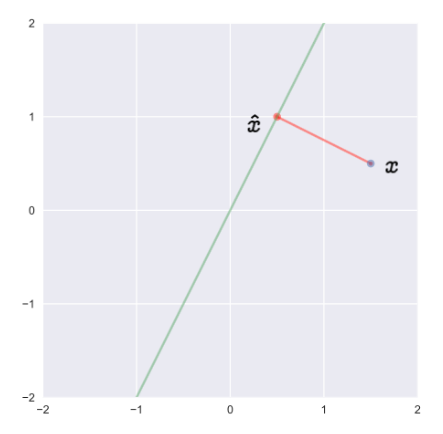
\includegraphics[width=0.5\textwidth]{pictures/proiezione.png}
	\caption{Proiezione di un punto su un sottospazio}
\end{figure}
\begin{itemize}
	\item Ogni osservazione $x$ viene assunta come "vicina" a una combinazione lineare di $\{\phi_1, \ldots, \phi_r\}$.
	\item Le colonne di $\Phi$ sono chiamate \textbf{componenti principali}.
	\item Il parametro $r<d$ è detto rango di riduzione, o dimensione del sottospazio.
	\item La funzione di loss associata è la distanza quadratica media tra i punti e le loro proiezioni:
	\[l(\Phi)=\frac{1}{n}||x-\hat{x}||_2^2\]
\end{itemize}
\begin{figure}[H]
	\centering
	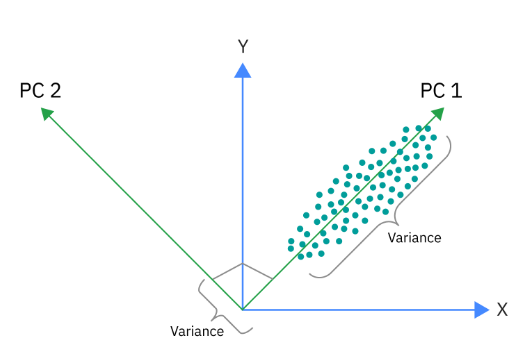
\includegraphics[width=0.5\textwidth]{pictures/pca.png}
	\caption{Esempio di PCA in 2D}
	\label{fig:pca}
\end{figure}
Un nuovo possibile sistema di coordinate (quello verde in figura \ref{fig:pca}) è quell dove gli assi sono uguali agli autovettori della matrice di covarianza del dataset.
Adesso immaginiamo di poter ruotare gli assi, in modo che nel nuovo sistema di coordinate la matrice di covarianza sia:
\[Cov(x,y)=\begin{bmatrix}
\sigma_1^2 & 0 \\
0 & \sigma_2^2
\end{bmatrix}\]
In questo modo le due variabili non sono correlate tra loro.
\begin{table}[H]
\centering

\begin{tabular}{lll}
\toprule
\textbf{Term} & \textbf{Expression} & \textbf{Description} \\
\midrule
Covariance matrix & $\Sigma = \frac{1}{n} X^{T} X$ & Describes the variability of the data \\
Eigenvector & $\phi_i$ & Principal direction (principal component) \\
Eigenvalue & $\lambda_i$ & Variance explained along $\phi_i$ \\
Component matrix & $\Phi = [\phi_1, \ldots, \phi_r]$ & Basis of the reduced subspace \\
Projection & $\hat{x} = \Phi \Phi^{T} x$ & Point projected onto the subspace \\
\bottomrule
\end{tabular}
\caption{Summary of key concepts in Principal Component Analysis (PCA).}
\end{table}
\noindent
Quindi la PCA è una trasformazione lineare che proietta il dataset in un nuovo sistema di coordinate, dove la prima coordinata ha più varianza,
ogni coordinata successiva ha varianza decrescente e tutte le coordinate sono ortogonali tra loro.
\\
In pratica trasformiamo un insieme di $x$ variabili correlate in un insieme di $p$ componenti principali non correlate.
\begin{enumerate}
	\item Creare la matrice $X$ di dimensione $K \times N$ dei dati, dove ogni riga è un'osservazione e ogni colonna una feature.
	\item Calcolare la matrice di covarianza $S$, basata su $X$. Questo cattura la ridondanza del dataset.
	\item Risolvere $S\underbar{e}=\lambda \underbar{e}$ per trovare gli autovettori $\underbar{e}$ e autovalori $\lambda$ di $S$. L'autovettore è una direzione, l'autovalore ci dice quanta varianze c'è nei dati in quella direzione.
	\item Risolvere $P=X\underbar{e}$ per calcolare le componenti principali ($N$ componenti)
\end{enumerate}
Tecnicamente, la quantità di varianza catturata dalla $i$-esima componente principale è misurata dall'auto valore $\lambda_i$.
La PCA è particolarmente utile quando le variabili nel dataset sono altamente correlate.
La correlazione indica che c'è ridondanza nei dati. A causa della ridondanza, la PCA può essere usata per ridurre le variabili originali in un numero minore di variabili (componenti principali), spiegando la maggior parte della varianza delle variabili originali.
\\
Gli autovalori possono essere usati per determinare il numero di PC da mantenere dopo la PCA.
\begin{itemize}
	\item Un autovalore $>1$ indica che le PC contano di più per la varianza che una delle variabili originali.
	\item In maniera alternativa, possiamo limitare il numero di componenti al numero che spiega una certa percentuale della varianza totale. 
\end{itemize}
Se voglio ad esempio spiegare almeno il $70\%$ dell'esempio in figura \ref{fig:pcaVarianza}, scelgo le prime 3 componenti.
\begin{figure}[H]
	\centering
	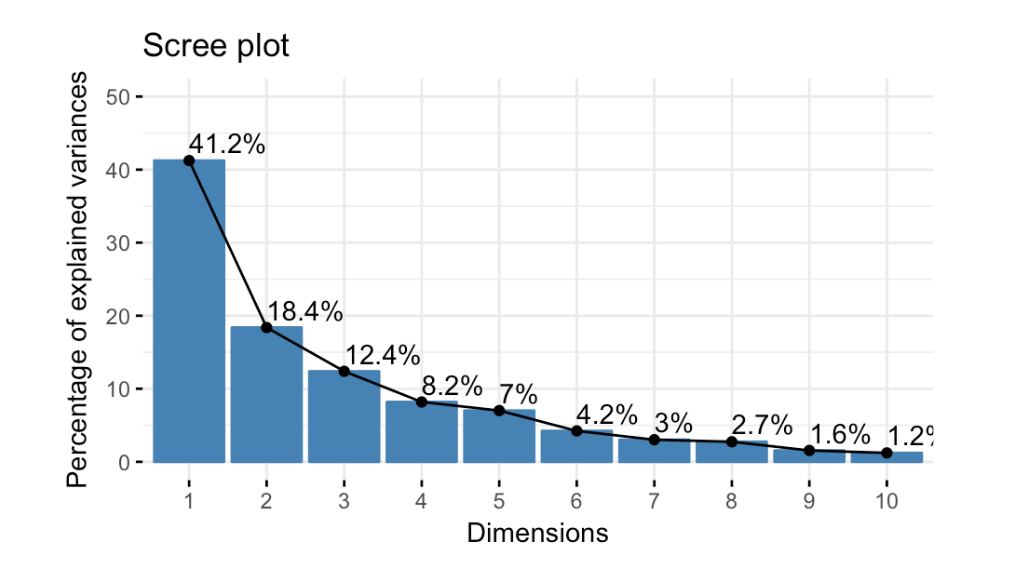
\includegraphics[width=0.7\textwidth]{pictures/pcaVarianza.png}
	\caption{Varianza spiegata dalle componenti principali}
	\label{fig:pcaVarianza}
\end{figure}

\end{document}